% Copyright 2005-2016 Airbus-EDF-IMACS-Phimeca
% Permission is granted to copy, distribute and/or modify this document
% under the terms of the GNU Free Documentation License, Version 1.2
% or any later version published by the Free Software Foundation;
% with no Invariant Sections, no Front-Cover Texts, and no Back-Cover
% Texts.  A copy of the license is included in the section entitled "GNU
% Free Documentation License".
\renewcommand{\nomfichier}{docref_C311_Form}
\renewcommand{\titrefiche}{FORM}

\Header

\MathematicalDescription{

  \underline{\textbf{Goal}} \vspace{2mm}

  The First Order Reliability Method is used under the following context: $\vect{X}$ is the input random vector and $\pdf$ its joint density probability function.\\

  Let us denote by $\vect{d}$ a determinist vector, $g(\vect{X}\,,\,\vect{d})$ the limit state function of the model, $\cD_f = \{\vect{X} \in \Rset^n \, / \, g(\vect{X}\,,\,\vect{d}) \le 0\}$ the  event considered here and {g(\vect{X}\,,\,\vect{d}) = 0} its boundary.\\

  The objective of FORM is to evaluate the probability content of the event $\cD_f$:
  \begin{equation}\label{PfX5}
    P_f = \Prob{g(\vect{X}\,,\,\vect{d})\leq 0}=   \int_{\cD_f}  \pdf\, d\vect{x}
  \end{equation}
  \vspace{2mm}

  \underline{\textbf{Principle}}

  \begin{center}
    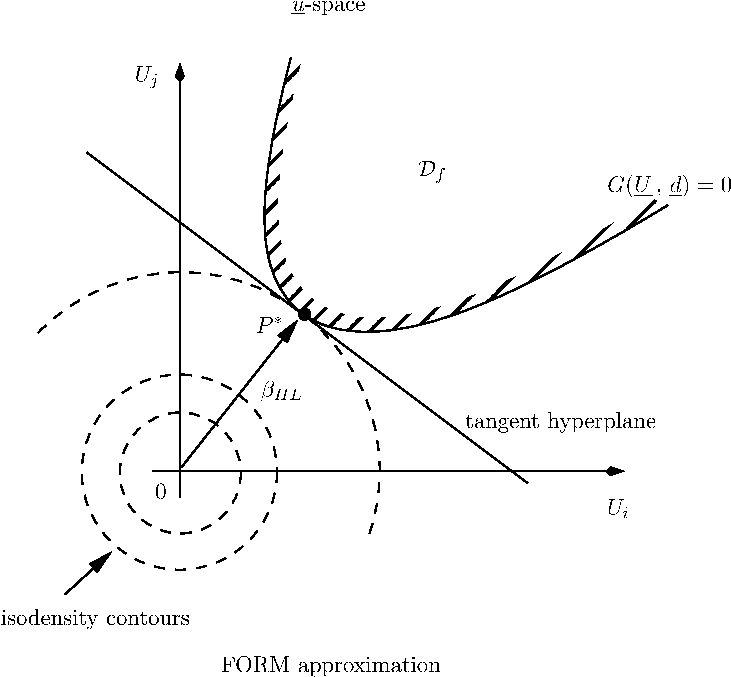
\includegraphics{Figures/FigureForm.pdf}
    \label{FORM}
  \end{center}

  The method proceeds in three steps :

  \begin{enumerate}
  \item Map the probabilistic model in terms of $\vect{X}$ thanks to an isoprobabilistic transformation (refer to \otref{docref_C311_TransIso}{Isoprobabilistic Transformation}) $T$ which is a diffeomorphism from $\supp(\vect{X})$ into $\Rset^n$, such that the distribution of the random vector $\vect{U}=T(\vect{X})$ has the following properties : $\vect{U}$ and $\mat{R}\,\vect{U}$ have the same distribution for all rotations $\mat{R}\in{\cS\cO}_n(\Rset)$.\\
    The usual isoprobabilistic transformations are the Generalized Nataf transformation (refer to \otref{docref_C311_TransIso_GeneralizedNataf}{Generalized Nataf}) and the Rosenblatt one (refer to \otref{docref_C311_TransIso_Rosenblatt}{Rosenblatt}).\\
    The mapping of the limit state function is $G(\vect{U}\,,\,\vect{d}) =  g(T^{-1}(\vect{U})\,,\,\vect{d})$. Then, the event probability $P_f$ rewrites :
    \begin{equation}\label{PfU3}
      P_f = \Prob{G(\vect{U}\,,\,\vect{d})\leq 0} = \int_{\Rset^n} \boldsymbol{1}_{G(\vect{u}\,,\,\vect{d}) \leq 0}\,f_{\vect{U}}(\vect{u})\,d\vect{u}
    \end{equation}
    where $f_{\vect{U}}$ is the density function of the distribution in the standard space : that distribution is spherical (invariant by rotation by definition). That property implies that $f_{\vect{U}}$ is a function of $||\vect{U}||^2$ only. Furthermore, we suppose that outside the sphere which tangents the limit state surface in the standard space, $f_{\vect{U}}$ is decreasing.

  \item Find the design point $\vect{u}^*$ which is the point verifying the event of maximum likelihood : the decreasing hypothesis of the standard distribution $f_{\vect{U}}$ outside the sphere which tangents the limit state surface in the standard space implies that the design point is the point on the limit state boundary the nearest to the origin of the standard space. Thus, $\vect{u}^*$ is the result of a constrained optimization problem.

  \item In the standard space, approximate the limit state surface in the standard space by a linear surface at the design point $ \vect{u}^*$. Then, the probability $P_f$ (\ref{PfU3}) where the limit state surface has been approximated by a linear surface (hyperplane) can be obtained exactly, thanks to the rotation invariance of the standard distribution $f_{\vect{U}}$ :
    \begin{equation}\label{PfFORM}
      P_{f,FORM}        =
      \left|
      \begin{array}{ll}
        E(-\beta_{HL}) & \mbox{if the origin of the $\vect{u}$-lies in the domain $\cD_f$} \\
        E(+\beta_{HL}) & \mbox{otherwise}
      \end{array}
      \right.
    \end{equation}

    where $\beta_{HL}$ is the Hasofer-Lind reliability index (refer to  \otref{docref_C311_ReliabIndex}{Reliability index}), defined as the distance of the design point $\vect{u}^*$ to the origin of the standard space and $E$ the marginal cumulative density function of the spherical distributions in the standard space.\\

    Let us recall here (refer to \otref{docref_C311_TransIso}{Isoprobabilistic Transformation}) that in the Rosenblatt standard space, random vectors follow the standard normal distribution (with zero mean, unit variance and unit correlation matrix), which implies that $E = \Phi$. In the Generalized Nataf standard space, random vectors follow some spherical distributions, with zero mean, unit variance, unit correlation matrix and which type $\psi$ is the one of the copula of the physical random vector $\vect{X}$ : in that case, $E$ is the 1D cumulative distribution function with zero mean, unit variance and which type is $\psi$.
  \end{enumerate}
}
{
  Here, the event considered is explicited directly from the limit state function $g(\vect{X}\,,\,\vect{d})$ : this is the classical structural reliability formulation.\\
  However, if the event is a threshold exceedance, it is useful to explicite the variable of interest $Z=\tilde{g}(\vect{X}\,,\,\vect{d})$, evaluated from the model $\tilde{g}(.)$. In that case, the event considered, associated to the threshold $z_s$ has the formulation: $\cD_f = \{ \vect{X} \in \Rset^n \, / \, Z=\tilde{g}(\vect{X}\,,\,\vect{d}) > z_s \}$
  and the limit state function is : $g(\vect{X}\,,\,\vect{d}) = z_s - Z = z_s - \tilde{g}(\vect{X}\,,\,\vect{d})$. $P_f$ is the threshold exceedance probability, defined as : $P_f     =       P(Z \geq z_s) = \int_{g(\vect{X}\,,\,\vect{d}) \le 0}  \pdf\, d\vect{x}$.
}


\Methodology{
  Within the global methodology, the First Order Reliability Method is used in the step C: "Uncertainty propagation" in the case of the evaluation of the probability of an event by an approximation method.\\
  It requires to have fulfilled the following steps beforehand:
  \begin{itemize}
  \item step A: identify of an input vector $\vect{X}$ of sources of uncertainties and an output variable of interest $Z=\tilde{g}(\vect{X},\vect{d})$, result of the model $\tilde{g}()$; identify a probabilistic criteria such as a threshold exceedance $Z > z_s$ or equivalently a failure event ${g(\vect{X}\,,\,\vect{d}) \le 0}$,
  \item step B: identify one of the proposed techniques to estimate a probabilistic model of the input vector $\vect{X}$,
  \item step C: select an appropriate optimization algorithm among those proposed.
  \end{itemize}

  The First Order Reliability Method provides the following results:
  \begin{itemize}
  \item the FORM probability calculated by eq.\ref{PfFORM},
  \item the importance factors associated to the event (refer to \otref{docref_Cprime31_FactImp}{Importance Factors} ),
  \item if asked by the user, the sensitivity factors associated to the event (refer to \otref{docref_Cprime31_FactSens}{Sensitivity Factors} ).
  \end{itemize}
}
{
  One is usually interested in the evaluation of a very small probability $P_f$ where the evaluation of the limit state function of the model requires computationally expensive subroutines. The FORM method has been designed specifically for such cases for which simulation techniques (see for instance \otref{docref_C321_MonteCarloStd}{standard sampling approach}) are computationally prohibitive.\\

  The quality of the results obtained by the First Order Reliability Method depends on:
  \begin{itemize}
  \item the quality of the optimization algorithm used to find the design point: it is important that the optimization converges towards the global minimum of the distance function %(refer to \otref{docu_C311_AlgoOpt}{Optimisation Algorithm}).
  \item the quality of the computation of the gradients of the limit state function. It is important to choose an optimization algorithm adapted to the model considered %((refer to \otref{docu_C311_AlgoOpt}{Optimisation Algorithm}).
  \item the quality of the design point in the $\vect{u}$-space. It has several fields:
    \begin{itemize}
    \item the shape of the limit state surface: the boundary is supposed to be well approximated        by a plane near the design point,
    \item the unicity of the design point in the $\vect{u}$-space: FORM is valid when there is only one point on the limit state surface at a distance minimal to the origin,
    \item the strongness of the design point: FORM is valid under the hypothesis that most of the contribution to $P_f$ is concentrated in the vicinity of the design point, which is the case both when around $\vect{P}^*$, the contribution decreases rapidly with the distance to $\vect{P}^*$ and when there is no local maximum with comparable density.
    \end{itemize}

    The first hypothesis can be checked by testing other method to evaluate $P_f$ : SORM (refer to
    \otref{docref_C311_Sorm}{SORM}) that takes into account the curvatures of the surface, or importance sampling techniques (refer to \otref{docref_C322_TI}{Importance sampling}) that makes no hypothesis on the shape of the surface.\\
    The unicity and the strongness of the design point can be checked thanks to the Strong Maximum Test (refer to \otref{docref_C312_StrongMaxTest}{Strong Max Test}).\\
    Accelerated sampling techniques such as directional sampling  (refer to \otref{docref_C322_SimuDir}{Directional sampling}) are also still valid if the unicity or strongness are doubtful.\\
    A limitation of FORM (or SORM) approximation is that it is generally impossible to quantify the approximation error. Although the method has been used satisfactorily in many circumstances, it is generally useful, if computationally possible, to validate Form/Som using at least one of the techniques above mentioned.
  \end{itemize}



  Let's note some usefull references:
  \begin{itemize}
  \item O. Ditlevsen and H.O. Madsen, 2004, "Structural reliability methods," Department of mechanical engineering technical university of Denmark - Maritime engineering, internet publication.
  \item R. Lebrun, A. Dutfoy, 2008, "A generalisation of the Nataf transformation to distributions with elliptical copula", Probabilistic Engineering Mechanics 24 (2009), pp. 172-178, doi:10.1016/j.probengmech.2008.05.001.
  \item R. Lebrun, A. Dutfoy, 2008, "Do Rosenblatt and Nataf isoprobabilistic transformations really differ?", submitted to Probabilistic  Engineering Mechanics in august 2008, under temptatively accepted so far.
  \item H. O. Madsen, Krenk, S., Lind, N. C., 1986, "Methods of Structural Safety," Prentice Hall.
  \end{itemize}
}
\Example{
  {\bf Example 1 }:
  Let's apply this method to the following analytical example which considers a cantilever beam, of Young's modulus E, length L, section modulus I. We apply a concentrated bending force at the other end of the beam. The vertical displacement $y$ of the extrême end is equal to :
  \begin{align*}
    y(E, F, L, I) = \displaystyle \frac{FL^3}{3EI}
  \end{align*}
  The objective is to propagate until $y$ the uncertainties of the variables $(E, F, L, I)$.\\
  The input random vector is $\vect{X} = (E, F, L, I)$, which probabilistic modelisation is (unity is not provided):
  \begin{align*}
    \left\{
    \begin{array}{lcl}
      E & = & Normal(50, 1) \\
      F & = & Normal(1, 1) \\
      L & = & Normal(10, 1) \\
      I & = & Normal(5, 1)
    \end{array}
    \right.
  \end{align*}
  The event considered is the threshold exceedance : $\cD_f = \{(E, F, L, I) \in \Rset^4 \, / \, y(E, F, L, I) \ge 3\}$
  We obtain the following results, where the Generalized Nataf transformation has been used :
  \begin{itemize}
  \item[$\bullet$] design point in the $\vect{x}$-space, $P^* = (E^* = 49.97,F^* = 1.842, l^* = 10.45,I^* = 4.668)$
  \item[$\bullet$] the generalized and Hasofer  reliability index : $\beta_g = \beta_{HL} = 1.009$
  \item[$\bullet$] the FORM probability : $P_{f,FORM} = 1.564e^{-1}$
  \end{itemize}


  {\bf Example 2 }: If we evaluate the FORM probability in the example described in \otref{docref_C311_TransIso_Rosenblatt}{Rosenblatt},  in the case where $\theta = 10$, $\lambda_1 = 1$ and $\lambda_2 = 3$ and where we considered the canonical order and its inverse of the Rosenblatt transformation, we obtain :
  \begin{equation}
    \left\{
    \begin{array}{lcl}
      \beta_{CanOrd} & = & 1.24 \\[0.5em]
      \beta_{InvOrd} & = & 1.17
    \end{array}
    \right.
  \end{equation}

  which leads to different FORM approximations of the failure probability:
  \begin{equation}
    \left\{
    \begin{array}{lcl}
      P^{FORM}_{CanOrd} & = & 1.07 \, 10^{-1} \\[0.5em]
      P^{FORM}_{InvOrd} & = & 1.22 \, 10^{-1}
    \end{array}
    \right.
  \end{equation}


}
